\chapter{Ausblick}
\label{cha:Ausblick}

\section{Frameworks}
In dem folgendem Kapitel soll die Auswahl der zu nutzenden Frameworks verargumentiert werden, jedoch sind die genannten Frameworks nur ein Ausschnitt der im Github Repository Diskutierten Produkte die im Netz verfügbar sind.
% Vue Native - PWA für full support
Für das Frontend gibt es eine Reihe an Javascript Frameworks die das Implementieren von PWA Funktionalitäten als auch den Export zu einer Nativen App erleichtern. Besonders bekannt sind dabei Vue und React Native. Beide bieten ähnliche Features. Auf Grund dessen, dass ich mehr Erfahrung mit Vue habe, wähle ich Vue Native. Diese Wahl basierd auf reinen persönlichen Präferenzen und der bekanntlich schnell erlernbaren Syntax und Semantik von Vue, sowie die Erfahrung die ich bereits mit Vue habe. Dieses Vorgehen der Auswahl eines Javascript Frameworks, ist die empfohlene Vorgehensweise unter Entwicklern.
% React Native / PWA als Alternative
% NoSQL vs SQL
Ob die Datenbank nach SQL oder dem NoSQL Schema aufgebaut sein soll, lässt sich nicht hundertprozentig beantworten. Jedoch als Best Practice gilt die Skalierbarkeit von Systemen und somit auch die Datenbanken, was sich am besten mit NoSQL realisieren lässt. Jedoch sind SQL Datenbanken besonders geeignet für die Dartstellung von Relationen, welche in diesem System besonders häufig vertreten sind. Das erwartete Wachstum des Systems und die damit steigenden Abfragen an das System, sowie die Implementierung von Empfehlungsalgorithmen, sprechen jedoch wieder für eine NoSQL Datenbank. Hier gibt es verschiedene Frameworks zur Auswahl. Für den lokalen Speicher ist man jedoch noch häufig abhängig von Google Produkten.
% ### SQL
%- Vorteile: 
%    - Geeignet für Sozial Media Applications
%        - Geeignet für die Darstellungen von Beziehungen
%    - Geeignet für Finanzsystem
%- Nachteile:
%    - Große Abfragen brauchen länger
%### NoSQL
%- Vorteile: 
%    - Geeignet bei vielen Lese/Schreibe Operationen
%    - Geeignet wenn schnelle Skalierung erforderlich ist
%    - Geeignet wenn viele Daten versendet/empfangen werden
%    - Geeignet für dynmaische Inhalte
%- Nachteile:
%    - Komplexeres Setup

\section{Disclaimer}
% Die Auswahl der Frameworks und die Gestaltungslösung ist nur eine Momentaufnahme basierend auf den schnell sich anpassenden Anforderungen an solche Systeme
Da sich die Anforderungen an Webseiten, Soziale Netzwerke und Applikationen stetig ändern, ist die Auswahl und die Erarbeitung der Gestaltungslösung und Frameworks nur eine Momentaufnahme dessen, was die Nutzer gemeinsam entwicklelt haben. Kommende Entwickler müssen sehr wahrscheinlich von Vorne beginnen um alle Anforderungen an Systeme wie diese nutzerzentriert zu erarbeiten. Das Einbringen von Guidelines, kann die Arbeit erleichtern, ergibt aber nicht immer die praktikabelste und ergonomischte Lösung.

\section{Mögliche folge Projekte}
% Peer to Peer lösung mit Lokalem oder Cloud Speicher einzelner Nutzer
Sofern technisch möglich, wäre ein spannedes folge Projekt die Umsetzung eines ähnlichen Systems auf Basis von Peer to Peer Kommunikation zwischen Client und Server als auch den Endgeräten. Die sich daraus resultierenden Synchronisationsprobleme könnten mit Hilfe von Blockchain oder offenen Frameworks für den lokalen Speicher lösen lassen. Die aktuellen Limitierungen des lokalen Speichers machen dieses Projekt jedoch zur Zeit nur eingeschränkt möglich.
% Framework bauen für eine Peer to Peer Lösung
Ein weiteres spannendes Projekt wäre die Umsetzung eines Frameworks für soziale Netzwerke, unabhängig von großen Unternehmen und komplett Open Source. Dabei müssen die genutzten Technologien ständig von der Community evaluiert werden, das Ergebnis wäre jedoch die Anreicherung des Marktes von Sozialen Netzwerken mit vielen neuen Produkten die sich nicht direkt an große Unternehmen binden und deren Position stärken.
% Stack Image für easy set up
Ein folge Projekt dafür wäre die Etablierung eines solchen Stacks als Image, welches sich mit Hilfe von Virtualisierungsprogrammen wie Docker schnell selber aufsetzen lässt und somit die Einstiegshürde für junge Entwickler sinkt.

\chapter{Schluss}
\label{cha:Schluss}

\section{Selbsteinschätzung (Bezug auf These)}


\section{Fazit in Zahlen (Umfragen)}
\begin{figure}[h] %!=overrides latex; h=here; t=top; b=bottom; p=special page for floating objects
    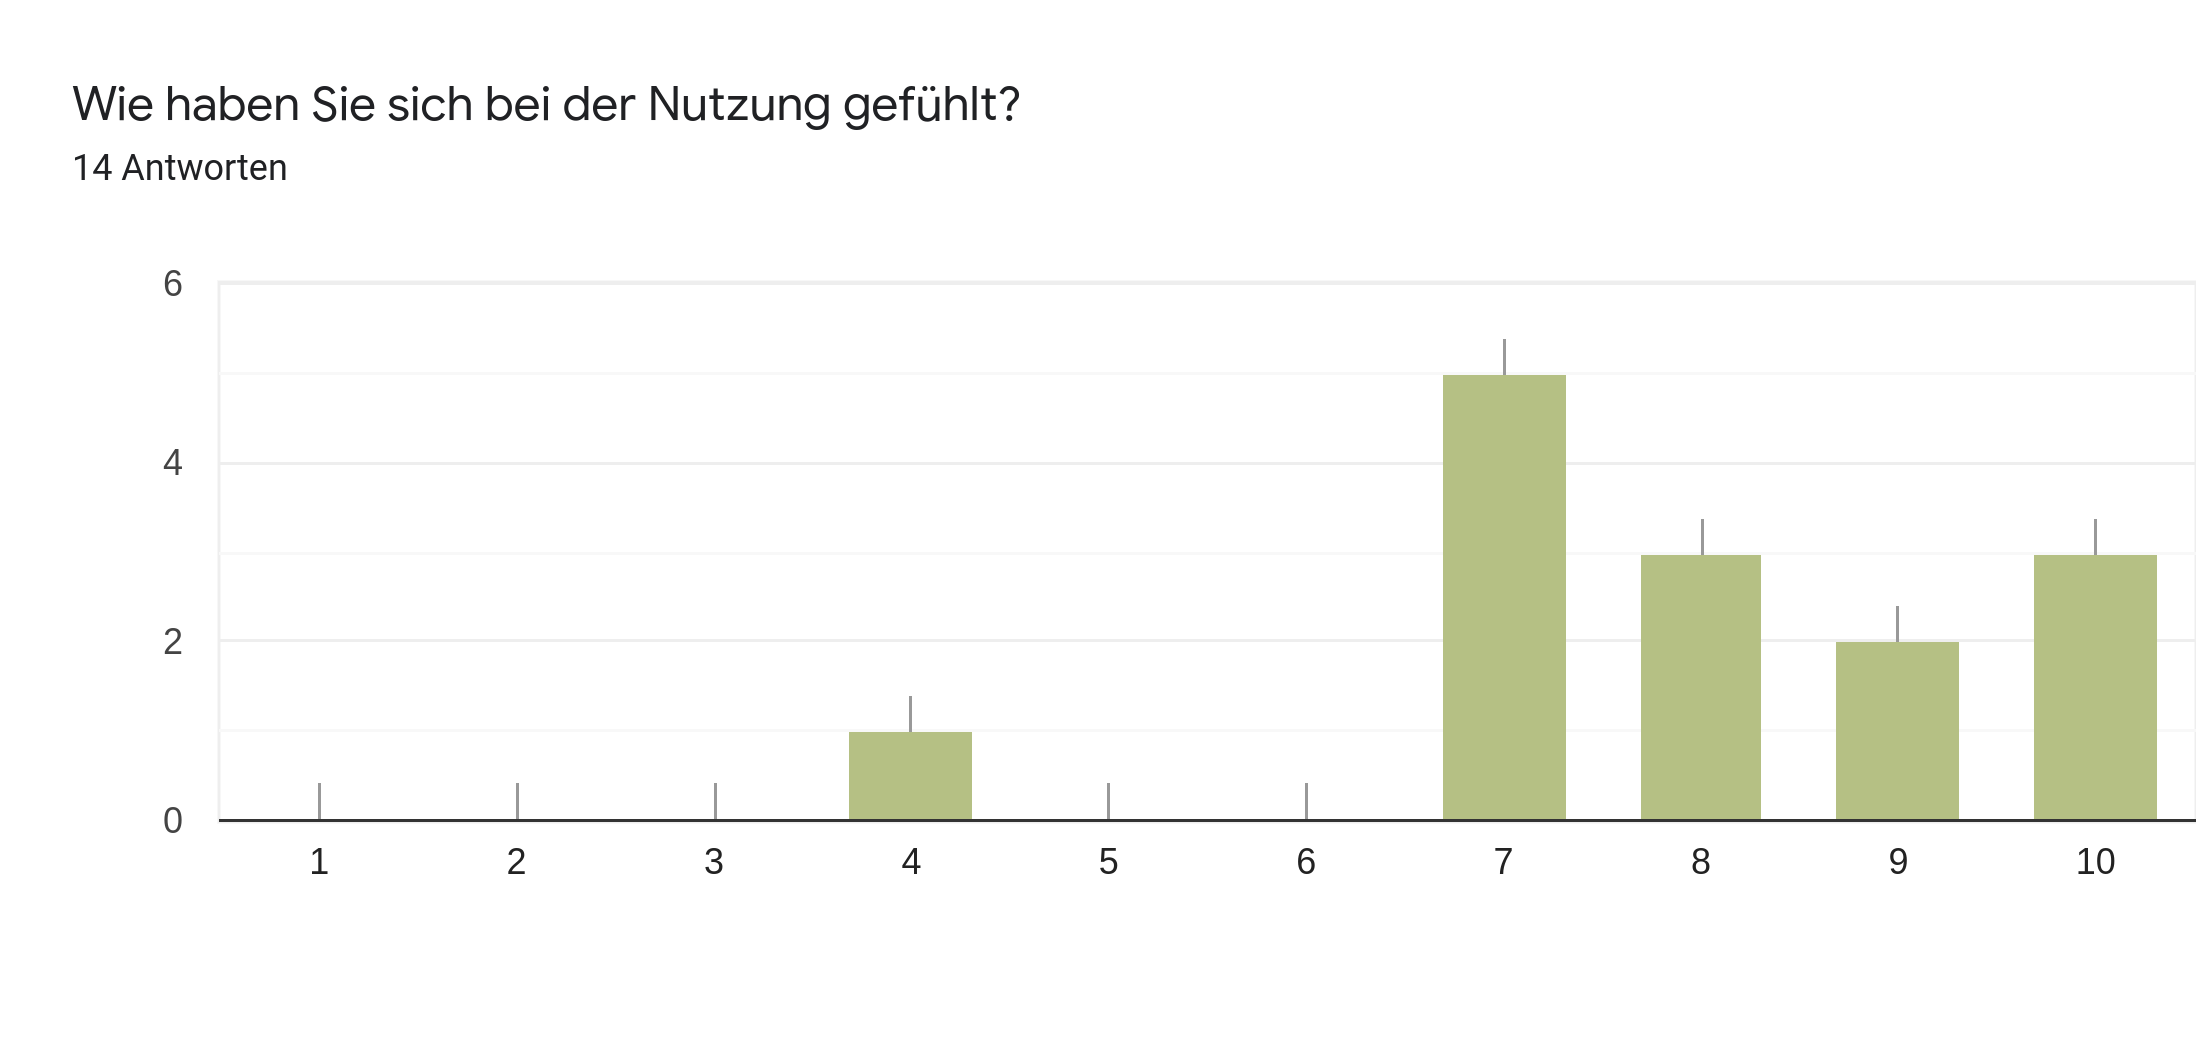
\includegraphics[width=1\textwidth]{images/PersonlichesEmpfinden.png}
    \caption[Evaluierung - 1 schlecht 10 sehr gut]{Evaluierung}
    \label{fig:personlicheEmpfindung}
\end{figure}
An der abschließenden Befragung potentieller Nutzer nahmen insgesamt 14 Personen teil. Dabei vielen die persönlichen Eindrücke der Nutzung großteilig positiv aus. Ein Prozent gab an eine subjektiv schlechte Erfahrung mit dem Prototypen gehabt zu haben. Ausgehend von den restlichen Bewertungen, scheint dies jedoch mit der Vertrautheit der älteren Personengruppen mit neuartigen digitalen Medien zu korrelieren. Die Erstellung eines Rezeptes wurden mit 42\% empfanden das Erstellen von Rezepten als einfach. Dagegen 14\% empfanden das angeleitete Erstellen eines Rezepts als schwer. Das finden von den eigenen Freunden und der privaten Rezepte bewerteten 57\% als einfach. 71\% gaben and, dass die Gestaltung der App ihren Erwartungen entspreche. 41\% jedoch gaben an, dass sie die Benutzung der App als ergnomisch oder intutiv bewerten würden. Dies lässt darauf schließen, dass in kommenden Iterationen an den User Stories weiter entwickelt werden sollte oder mehr Nutzerüberflächen erklärt werden müssen. Ein weiteres Problem ist die Differenzierung von gespeicherten und favorisierten Rezepten. Diese Unterteilung wurde von 14\% Prozent nicht verstanden und kritisiert. Ein weiterer wichtiger Punkt ist die Kritik an der Schriftgröße. Diese wurden zwar nach den Guidelines und Fibunacci Skalen erstellt, der Evaluation ist jedoch zu entnehmen, dass diese zu klein angesetzt sind und vergrößert werden müssen um in der Praktik lesbar zu sein. Die Übersicht über die Vorgänger und Original Rezepte wurde ebenfalls als nicht sonderlich wichtig bewertet und soll weiter unten an das Rezept angehangen werden, da es von dem eigentlich Rezept ablenkt. Auch das Deaktivieren und Ersetzen der Benachrichtigungsicons wurde kritisiert, da hier wohl die Bedeutung des Wechsels unklar ist. Im Gegensatz dazu wurde die Wahl der Icons als auch die Gestaltung von 42\% als positiv befunden. 

\section{(Persönliches Statement)}
% wird fortlaufend auf der Basis benutzerzentrierter Evaluierung vorangetrieben